\chapter{种群与种群统计学}\label{ch:b1:populations}

一瓶酵母起初有一百万个\omterm{def:b1:cell-unit-of-life:cell}{细胞}，十六小时后
\omterm{def:b1:cell-unit-of-life:cell}{细胞}增至六千万个并停止增长；一群岛上的鹿
每年增长十分之一，直到冬季食物耗尽为止；
北方针叶林的猞猁每十年数量升高又骤降一次，比
它们所捕食的野兔晚一年。每个都是一个\emph{\omterm{def:b1:populations:population}{种群}}——即
同一地点同一物种的个体——且每个\omterm{def:b1:populations:population}{种群}都服从
可以写下来的数量规律。本章介绍\omterm{def:b1:populations:population}{种群}如何计数、
其出生与死亡如何列表统计、两种增长方程、
抑制\omterm{def:b1:populations:population}{种群}数量的各种力量，以及同样的数量规律
对人类这一物种说明了什么。

\section{种群计数}

\begin{definition}[种群、密度与分布格局]\label{def:b1:populations:population}
\index{种群}\index{种群密度}
\emph{种群}是指生活在给定区域、在给定时间内
并能相互交配的同一物种个体的集合。其
\emph{种群大小} $N$ 为个体数目；其\emph{密度}为
单位面积或体积内的个体数；其\emph{分布格局}是
个体的间距格局——资源或群居生活使其聚集时为\emph{集群分布}
（如鹿群、鱼群、植物斑块），\emph{均匀分布}指个体
相互排斥（如占域鸟类、为争夺
水分而竞争的荒漠灌木），两者均不起作用时为\emph{随机分布}。种群还具有一个
\emph{年龄结构}、\emph{性别比例}，以及出生、死亡、
迁入和迁出的速率，这些速率的平衡即为增长。
\end{definition}

\begin{method}[种群数量估计]\label{met:b1:populations:counting}
\index{标记重捕法}
\begin{enumerate}
  \item 固着或移动缓慢的生物：在随机放置的、面积已知的\emph{样方}中计数，
        然后以平均密度乘以
        总面积；样方间的离散程度给出精度，
        并揭示分布格局。
  \item 可移动的动物：\emph{标记重捕法}。捕获 $M$
        个体，做标记后放回；随后捕获 $C$ 个，其中
        $R$ 个带有标记。若带标记者与其余个体自由混合，且
        期间没有任何变化，则第二次捕获中带标记者的比例等于
        \omterm{def:b1:populations:population}{种群}中带标记者的比例，即 $R/C = M/N$，因此
        $N \approx MC/R$（林肯–皮特森估计）。
  \item 检验假设：两次捕获之间没有出生、死亡或迁移，
        标记既不脱落，也不改变
        个体的行为，且各个体被捕获的概率相等。每项假设不成立都会
        使 $N$ 朝可预测的方向产生偏差。
  \item 无法直接计数时，可利用间接迹象：粪便、
        足迹、叫声、巢穴，以及一升池塘水中的 \omterm{def:b1:nucleic-acids:chain}{DNA}。
\end{enumerate}
\end{method}

\begin{example}[草地中的田鼠]\label{ex:b1:populations:voles}
在一公顷草地中捕获、做标记并放回六十只田鼠；
三个夜晚之后又捕获八十只，其中十二只带有标记：
$N \approx 60\times 80/12 = 400$ 只田鼠，每一百平方米四只。
若带标记的田鼠已经知道陷阱中有食物，则它们
更易被捕获，$R$ 偏大，$N$ 被低估；若标记
使田鼠远离陷阱，则偏差方向相反。
\end{example}

\section{种群统计学：按年龄划分的出生与死亡}

\begin{definition}[生命表]\label{def:b1:populations:lifetable}
\index{生命表}\index{存活率}
\emph{生命表}追踪同时出生的一批个体
的一生。对每个年龄 $x$，记录 $l_x$，即
\emph{存活率}——该批个体中仍活到年龄 $x$
时的比例——以及 $m_x$，即\emph{繁殖力}——年龄为 $x$ 的
雌性所生雌性后代的平均数。由此可得各年龄之间的死亡率
$q_x = 1 - l_{x+1}/l_x$；\emph{净繁殖
率} $R_0 = \sum_x l_x m_x$，即一个新生雌性
一生中平均将产生的雌性后代数；\emph{世代时间}
$T = \sum_x x\,l_x m_x / R_0$，即这些雌性后代的
母亲的平均年龄。$R_0 > 1$ 的\omterm{def:b1:populations:population}{种群}增长，$R_0 < 1$
的\omterm{def:b1:populations:population}{种群}下降；经过一个世代，\omterm{def:b1:populations:population}{种群}数量乘以 $R_0$。
\end{definition}

\begin{proposition}[存活曲线的三种类型]\label{prop:b1:populations:survivorship}
以 $\log l_x$ 对年龄作图，可得三种类型的曲线。\emph{I
型}：多数个体存活至老年，并在较窄的年龄范围内死亡
（大型哺乳动物、富裕国家的人类）。\emph{II 型}：各年龄的死亡概率
恒定，在对数坐标上呈一条直线。
（许多鸟类、蜥蜴与啮齿动物）。\emph{III 型}：幼体死亡率极高，
少数存活下来的个体则寿命很长（牡蛎、鱼类、
大多数植物与昆虫）。曲线形状取决于\omterm{def:b1:organism-environment:organism}{生物体}的生活方式：
一个物种若对每个后代投入很少、后代数量很多，
则具 III 型曲线；对少数后代各投入很多者，则为 I 型。
\end{proposition}

\begin{omfigure}
\begin{tikzpicture}
\begin{semilogyaxis}[
  width=0.86\linewidth, height=6.2cm,
  axis x line=bottom, axis y line=left,
  xmin=0, xmax=100, ymin=1, ymax=1200,
  xlabel={年龄（占最长寿命的\%）}, ylabel={每 1000 个出生个体的存活数},
  xlabel style={font=\small, at={(axis description cs:0.5,-0.12)}, anchor=north},
  ylabel style={font=\small},
  tick label style={font=\small}, xtick={0,25,50,75,100}, ytick={1,10,100,1000}, log ticks with fixed point,
  legend style={font=\small, at={(0.03,0.05)}, anchor=south west, draw=none},
  clip=false,
]
\addplot[very thick, omDef, smooth] coordinates {(0,1000) (20,990) (40,970) (60,900) (75,700) (85,400) (92,150) (97,30) (100,1)};
\addlegendentry{I 型：哺乳动物、人类}
\addplot[very thick, omProp, domain=0:100, samples=20] {1000*exp(-0.069*x)};
\addlegendentry{II 型：鸟类、啮齿动物}
\addplot[very thick, omThm, smooth] coordinates {(0,1000) (3,100) (10,15) (25,6) (50,4) (75,2.5) (100,1)};
\addlegendentry{III 型：鱼类、牡蛎、大多数植物}
\end{semilogyaxis}
\end{tikzpicture}

{\small 三种存活曲线，均采用对数尺度。
I 型晚死亡，III 型早死亡，II 型以恒定
速率死亡；每条曲线都是一部以线条写成的生命史。}
\end{omfigure}

\begin{omfigure}
\begin{tikzpicture}[font=\footnotesize, line cap=round]
  % two age pyramids: growing (left) and stable (right)
  \foreach \i/\m/\f in {0/4.0/3.8, 1/3.4/3.3, 2/2.8/2.7, 3/2.2/2.2, 4/1.6/1.7, 5/1.1/1.2, 6/0.7/0.8, 7/0.35/0.5} {
    \fill[omDef!55] (-\m,0.5*\i) rectangle (0,0.5*\i+0.42);
    \fill[omThm!45] (0,0.5*\i) rectangle (\f,0.5*\i+0.42);
  }
  \node[anchor=north, align=center] at (0,-0.15) {增长型种群 \\（幼体众多）};
  \foreach \i/\m/\f in {0/1.6/1.5, 1/1.7/1.6, 2/1.8/1.7, 3/1.8/1.8, 4/1.7/1.8, 5/1.5/1.7, 6/1.1/1.4, 7/0.6/0.9} {
    \fill[omDef!55] (8.8-\m,0.5*\i) rectangle (8.8,0.5*\i+0.42);
    \fill[omThm!45] (8.8,0.5*\i) rectangle (8.8+\f,0.5*\i+0.42);
  }
  \node[anchor=north, align=center] at (8.8,-0.15) {稳定或老化种群 \\（各年龄组数量均匀）};
  \foreach \i/\l in {0/0--9, 2/20--29, 4/40--49, 6/60--69} { \node[anchor=east, font=\scriptsize] at (-4.3,0.5*\i+0.21) {\l}; }
  \node[anchor=south, omDef!70!black] at (-2.0,4.1) {雄性}; \node[anchor=south, omThm!80!black] at (2.0,4.1) {雌性};
\end{tikzpicture}

{\small 年龄金字塔：各年龄组的个体数，
雄性在左，雌性在右。底部宽广表示幼体众多，
\omterm{def:b1:populations:population}{种群}将继续增长；各年龄组数量均匀表示\omterm{def:b1:populations:population}{种群}趋于更替；底部狭窄
则表示\omterm{def:b1:populations:population}{种群}下降。}
\end{omfigure}

\begin{example}[一个鹿群的生命表]\label{ex:b1:populations:deer}
在一千只幼鹿中，六百只活到第一个生日，
此后存活者每年损失十分之一，直到很少有个体能活过
九岁；雌鹿自两岁起繁殖，盛年时每年约产 0.8 只雌性后代。
将 $l_x m_x$ 求和，得 $R_0 \approx 1.5$：每只雌鹿
平均留下一只半雌性后代，鹿群每代增长一半，
一代约四年——即每年增长百分之十一，
直到某种因素将其制止。
\end{example}

\section{增长}

\begin{theorem}[指数增长]\label{thm:b1:populations:exponential}
\index{指数增长}\index{内禀增长率}
若\omterm{def:b1:populations:population}{种群}的人均出生率 $b$ 与人均死亡率 $d$ 为
常数，则\omterm{def:b1:populations:population}{种群}按与其大小成正比的速率增长，
\[
\frac{\dd N}{\dd t} = rN, \qquad r = b - d, \qquad N(t) = N_0\,e^{rt},
\]
其中 $r$ 为\emph{内禀增长率}。\omterm{def:b1:populations:population}{种群}每经过
$\ln 2/r$ 时间倍增一次；$r = \qty{0.11}{yr^{-1}}$ 的\omterm{def:b1:populations:population}{种群}在
\qty{6.3}{yr} 内倍增，$r = \qty{0.5}{h^{-1}}$ 的\omterm{def:b1:populations:population}{种群}则在 \qty{83}{min} 内倍增。
由\omterm{def:b1:populations:lifetable}{生命表}可得 $r \approx \ln R_0 / T$。
\end{theorem}
\begin{proof}
在很短的时间间隔 $\dd t$ 内，出生数为 $bN\,\dd t$，死亡数为
$dN\,\dd t$，故 $\dd N = (b - d)N\,\dd t$；方程
$\dd N/\dd t = rN$ 的解为 $N_0 e^{rt}$（$e^{rt}$ 的导数为
$re^{rt}$）。倍增时令 $e^{rt} = 2$，得 $t = \ln 2/r$。在
一代 $T$ 内，\omterm{def:b1:populations:population}{种群}数量乘以 $R_0 = e^{rT}$，
于是 $r = \ln R_0/T$。
\end{proof}

\begin{theorem}[逻辑斯谛增长]\label{thm:b1:populations:logistic}
\index{逻辑斯谛增长}\index{环境容纳量}
若人均增长率随\omterm{def:b1:populations:population}{种群}趋近
\emph{\omterm{thm:b1:populations:logistic}{环境容纳量}} $K$ 而线性下降——即\omterm{def:b1:organism-environment:organism}{环境}
所能承载的规模——
\[
\frac{\dd N}{\dd t} = rN\left(1 - \frac{N}{K}\right), \qquad
N(t) = \frac{K}{1 + \dfrac{K - N_0}{N_0}\,e^{-rt}} .
\]
$N \ll K$ 时增长近似为指数式，在 $N = K/2$ 时最快
（此时 $\dd N/\dd t = rK/4$），在 $N = K$ 时增长消失，\omterm{def:b1:populations:population}{种群}
逐渐趋于平台，呈 S 形曲线。
\end{theorem}
\begin{proof}
将方程写成 $\dd N/[N(1 - N/K)] = r\,\dd t$，并将
左边拆为 $\dd N/N + \dd N/(K - N)$，积分得
$\ln[N/(K - N)] = rt + \text{常数}$，并解出 $N$，使 $N(0) =
N_0$ 即得公式。对 $rN(1 - N/K)$ 关于
$N$ 求导并令其为零，得极大值点 $N = K/2$。
\end{proof}

\begin{omfigure}
\begin{tikzpicture}
\begin{axis}[
  width=0.86\linewidth, height=6.4cm,
  axis x line=bottom, axis y line=left,
  xmin=0, xmax=18, ymin=0, ymax=800,
  xlabel={时间 (h)}, ylabel={每毫升酵母细胞数 ($\times 10^5$)},
  xlabel style={font=\small, at={(axis description cs:0.5,-0.12)}, anchor=north},
  ylabel style={font=\small},
  tick label style={font=\small}, xtick={0,4,8,12,16}, ytick={0,200,400,600,800},
  legend style={font=\small, at={(0.03,0.97)}, anchor=north west, draw=none},
  clip=false,
]
\addplot[very thick, omDef, domain=0:18, samples=100] {660/(1+65*exp(-0.53*x))};
\addlegendentry{逻辑斯谛曲线，$K = 660$，$r = \qty{0.53}{h^{-1}}$}
\addplot[thick, dashed, omThm, domain=0:9, samples=50, restrict y to domain=0:800] {10*exp(0.53*x)};
\addlegendentry{相同 $r$ 的指数增长曲线}
\addplot[only marks, mark=*, mark size=1.8pt, omDef!70!black] coordinates {(0,10) (2,29) (4,71) (6,175) (8,351) (10,513) (12,595) (14,641) (16,656)};
\draw[dashed, gray] (axis cs:0,660) -- (axis cs:18,660); \node[font=\scriptsize, anchor=south east] at (axis cs:18,662) {$K$};
\draw[dashed, gray] (axis cs:0,330) -- (axis cs:7.9,330); \node[font=\scriptsize, anchor=west] at (axis cs:8.2,300) {$K/2$ 处增长最快};
\end{axis}
\end{tikzpicture}

{\small 每两小时计数一次的酵母培养物（数据点）、拟合其上的逻辑斯谛
曲线，以及若无上限时本应遵循的
\omterm{thm:b1:populations:exponential}{指数增长}曲线。两者在前六小时基本吻合，之后逐渐分开。}
\end{omfigure}

\begin{proposition}[密度制约]\label{prop:b1:populations:densitydependence}
\index{密度制约}
随着密度升高，增长减缓，原因在于人均出生率下降
或拥挤使死亡率上升：人均食物减少，
领地不再可用，废物与疾病积累，
捕食者聚集。这些\emph{密度制约}因素将
\omterm{def:b1:populations:population}{种群}调节至 $K$ 附近。\emph{非密度制约}因素——霜冻、
洪水、火灾、干旱——不论\omterm{def:b1:populations:population}{种群}数量多少都会杀死一部分个体，
无法起调节作用，只能造成扰动；许多昆虫的\omterm{def:b1:populations:population}{种群}
主要受天气支配，从不接近\omterm{thm:b1:populations:logistic}{环境容纳量}。
\end{proposition}
\begin{proof}[证据]
高斯（1934）在每日更换培养基的试管中培养\emph{Paramecium}：
计数值遵循逻辑斯谛曲线，趋于一个由食物决定的平台，
食物加倍则平台加倍。珀尔（1927）发现相同情形，
瓶中果蝇同样如此，卡尔森（1913）则在酵母中观察到。在野外，
岛上的歌雀每窝卵数减少，
繁殖\omterm{def:b1:populations:population}{种群}较大时损失的幼体更多，且领地数目
限制了繁殖个体的数量；移除鸟类后，
由先前被排除在外的过剩个体加以替补。
\end{proof}

\begin{definition}[生活史策略]\label{def:b1:populations:rK}
\index{r 选择}\index{K 选择}
物种在两个极端之间各有其位置。
\emph{$r$ 选择}物种——杂草、蚜虫、小鼠、大多数鱼类——
其特征是 $r$ 值高：发育早，产生大量小型后代，
对每个后代投入很少，寿命短，利用新出现的或受干扰的
生境，在竞争到来之前完成繁殖，具有 III 型存活曲线。
\emph{$K$ 选择}物种——橡树、大象、信天翁——
其特征是在 $K$ 附近维持\omterm{def:b1:populations:population}{种群}：发育晚，产生少量大型
后代，并加以照料，寿命长，在拥挤、
稳定的生境中竞争力强，具有 I 型存活曲线。多数物种兼具两者，
这些名称标示的是这一尺度的两端。
\end{definition}

\section{波动与调节}

\begin{proposition}[捕食者与猎物的循环]\label{prop:b1:populations:cycles}
\index{种群循环}
有些\omterm{def:b1:populations:population}{种群}不会趋于稳定，而是振荡。北方森林中的雪兔
及以其为食的猞猁一同升降，
周期约为十年，猞猁比雪兔滞后一两年：
雪兔多则养活许多猞猁，猞猁多则把雪兔吃得减少，
雪兔稀少则猞猁挨饿，猞猁稀少则雪兔得以恢复。这一循环
一部分由捕食者驱动，一部分由雪兔自身的食物驱动，其
食物在过度啃食后的恢复需要数年；耦合的捕食者—猎物
模型（见\cref{ch:b1:species-interactions}）可由两个方程再现这种
振荡。
\end{proposition}
\begin{proof}[证据]
一家贸易公司的毛皮收购记录，从 1840 年代起
保存了九十年，记录了每年运入的猞猁与雪兔皮张数，
覆盖一个次大陆：两组数据都每九到十年出现一次峰值，
猞猁峰值滞后于雪兔，跨越九个完整周期。此后的野外研究
将雪兔与捕食者隔开或给予额外食物，表明
去除任一因素都会使周期减弱，两者同时去除，
周期即告消失。
\end{proof}

\begin{omfigure}
\begin{tikzpicture}
\begin{axis}[
  width=0.9\linewidth, height=6.0cm,
  axis x line=bottom, axis y line=left,
  xmin=1845, xmax=1935, ymin=0, ymax=160,
  xlabel={年份}, ylabel={毛皮交易量（千张）},
  xlabel style={font=\small, at={(axis description cs:0.5,-0.12)}, anchor=north},
  ylabel style={font=\small},
  tick label style={font=\small, /pgf/number format/1000 sep=}, xtick={1850,1870,1890,1910,1930}, ytick={0,50,100,150},
  legend style={font=\small, at={(0.97,0.97)}, anchor=north east, draw=none},
  clip=false,
]
\addplot[very thick, omProp, smooth] coordinates {(1845,20) (1848,50) (1851,120) (1853,40) (1856,15) (1859,60) (1862,140) (1864,60) (1867,20) (1870,50) (1873,100) (1876,30) (1879,12) (1882,70) (1885,150) (1888,40) (1891,20) (1894,50) (1897,100) (1900,30) (1903,15) (1906,60) (1909,120) (1912,30) (1915,15) (1918,50) (1921,110) (1924,40) (1927,15) (1930,60) (1933,100)};
\addlegendentry{雪兔}
\addplot[very thick, omDef, smooth] coordinates {(1845,10) (1849,20) (1852,45) (1855,20) (1858,8) (1861,25) (1864,60) (1866,25) (1869,10) (1872,30) (1875,40) (1878,15) (1881,10) (1884,40) (1887,70) (1890,20) (1893,10) (1896,30) (1899,45) (1902,15) (1905,8) (1908,35) (1911,55) (1914,15) (1917,8) (1920,30) (1923,50) (1926,15) (1929,10) (1932,30) (1935,45)};
\addlegendentry{猞猁}
\end{axis}
\end{tikzpicture}

{\small 北方森林各贸易站逐年收到的雪兔与猞猁皮张数
（经平滑处理）。两者周期约为十年，
猞猁比雪兔滞后一两年。}
\end{omfigure}

\begin{omfigure}
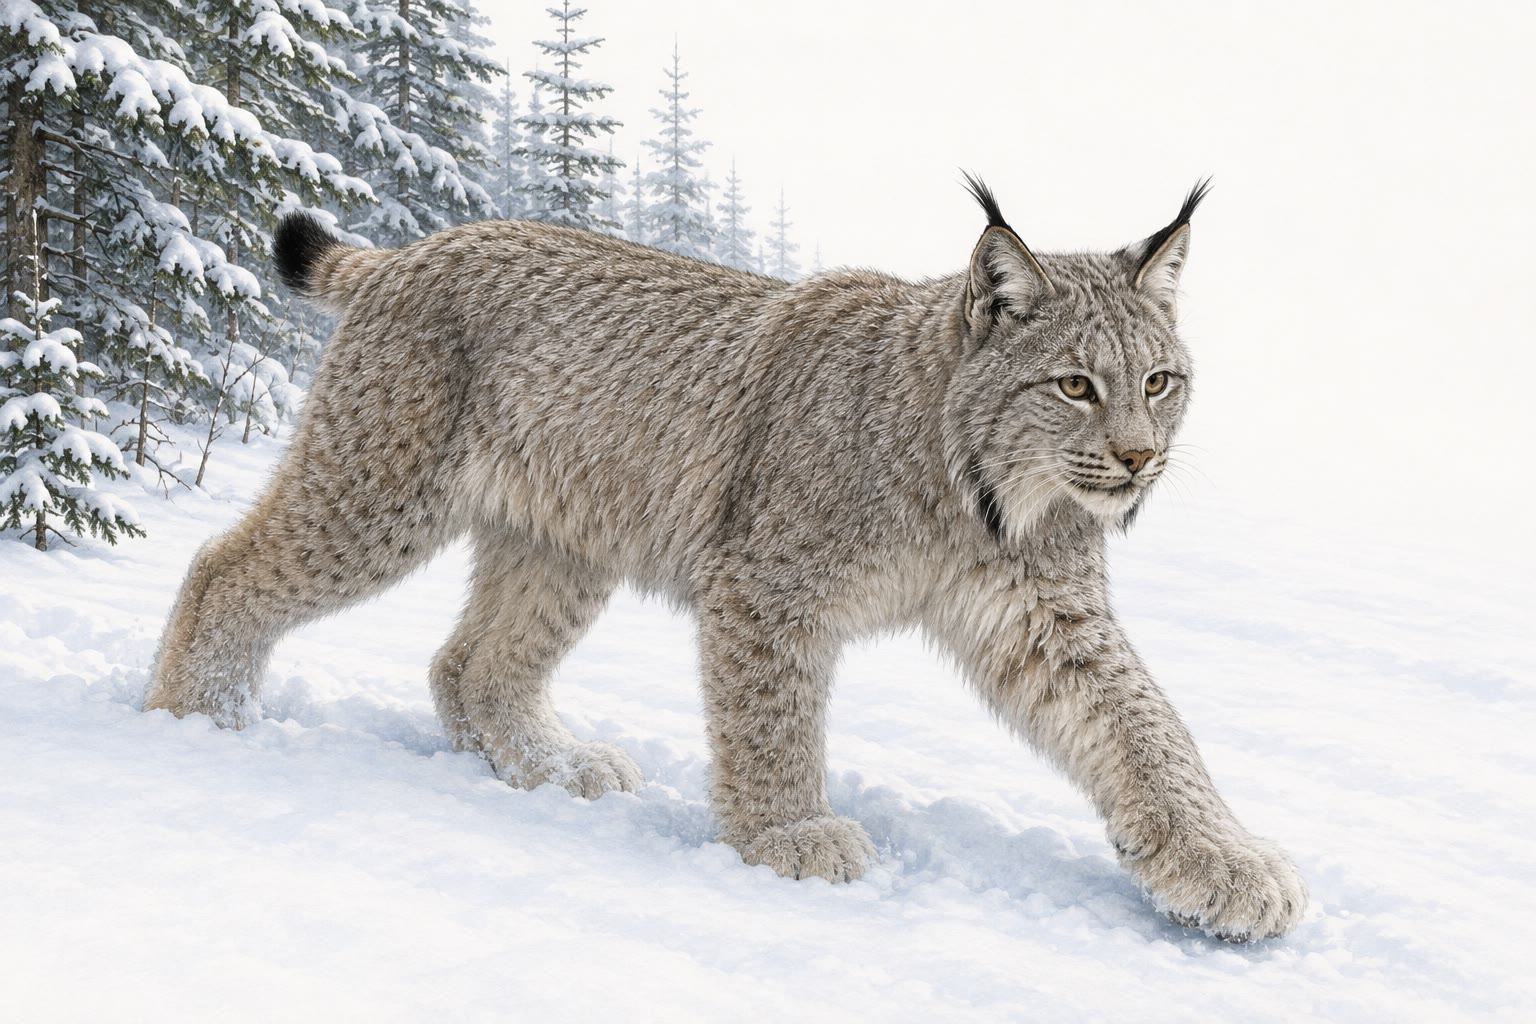
\includegraphics[width=0.52\linewidth]{images/book3/ai/b3-25-lynx-snow.jpg}

{\small 北方针叶林中的一只猞猁。其数量随雪兔变化，
存在滞后：捕食者的周期就是猎物周期的延迟。}
\end{omfigure}

\begin{example}[人类这一物种]\label{ex:b1:populations:humans}
人口用了全部历史时期才达到十亿，约在
1800 年左右，再用两个世纪才达到八十亿。其增长率
在 1960 年代达到峰值，接近每年 \qty{2}{\%}（35 年翻一番），此后
已降至 \qty{1}{\%} 以下，并非死亡所致，而是出生减少：
在儿童死亡率下降、女性接受教育的地方，家庭规模
在一代人之内缩小，年龄金字塔由三角形变为
柱形。$R_0$ 的计算方法同样适用于人类；变化的是 $m_x$。
\end{example}

\section{练习}

\begin{exercise}[$\star$]\label{exo:b1:populations:1}
定义\omterm{def:b1:populations:population}{种群}、密度与分布格局，并举出
每种分布格局的一个例子。
\end{exercise}

\begin{exercise}[$\star$]\label{exo:b1:populations:2}
定义 $l_x$、$m_x$、$R_0$ 和 $T$，并说明 $R_0 = 1$ 意味着什么。
\end{exercise}

\begin{exercise}[$\star$]\label{exo:b1:populations:3}
根据\omterm{def:b1:populations:lifetable}{存活率}图，III 型队列中
有多大比例的个体能存活过寿命的前十分之一？I 型队列中，
有多大比例能活到寿命的四分之三？
\end{exercise}

\begin{exercise}[$\star$]\label{exo:b1:populations:4}
写出\omterm{thm:b1:populations:exponential}{指数增长}方程和逻辑斯谛方程，并说明 $r$ 和 $K$
的含义。
\end{exercise}

\begin{exercise}[$\star\star$]\label{exo:b1:populations:5}
某细菌培养物的\omterm{def:b1:cell-unit-of-life:cell}{细胞}数由每毫升 $10^4$ 增至 $10^7$，
历时 \qty{5}{h}。求 $r$ 和倍增时间。
\end{exercise}

\begin{exercise}[$\star\star$]\label{exo:b1:populations:6}
某\omterm{def:b1:populations:lifetable}{生命表}：$l_x = 1, 0.5, 0.3, 0.1, 0$ 对应年龄 0 至 4；$m_x = 0,
1, 2, 2, 0$。求 $R_0$、$T$ 和 $r$，并
判断\omterm{def:b1:populations:population}{种群}是否增长。
\end{exercise}

\begin{exercise}[$\star\star$]\label{exo:b1:populations:7}
在池塘中标记并放回 50 条鱼；一周后
捕获 70 条，其中 7 条有标记。估计 $N$。若其中有标记的鱼有 10 条因
捕捉处理而死亡，估计值是偏高还是偏低？偏差多少？
\end{exercise}

\begin{exercise}[$\star\star$]\label{exo:b1:populations:8}
某逻辑斯谛\omterm{def:b1:populations:population}{种群}的 $K = 1000$ 且 $r = \qty{0.2}{yr^{-1}}$。
求 $\dd N/\dd t$ 在 $N = 100$、$500$ 和 $900$ 时的值，以及每年
可收获而不致\omterm{def:b1:populations:population}{种群}下降的最大数量。
\end{exercise}

\begin{exercise}[$\star\star$]\label{exo:b1:populations:9}
将下列生物归为 $r$ 选择或 $K$ 选择，各列两个性状：蒲公英、
大象、鳕鱼、大猩猩、家蝇。
\end{exercise}

\begin{exercise}[$\star\star\star$]\label{exo:b1:populations:10}
根据酵母图，由前两点估计 $r$，并由
最后一点估计 $K$，再用逻辑斯谛公式预测 \qty{8}{h} 时的 $N$，
并与计数比较。增长速率在何时
最高？此时的值是多少？
\end{exercise}

\begin{exercise}[$\star\star\star$]\label{exo:b1:populations:11}
试利用方程解释，为何非密度制约因素
虽能使\omterm{def:b1:populations:population}{种群}减少，却不能调节\omterm{def:b1:populations:population}{种群}，
而受天气支配的昆虫\omterm{def:b1:populations:population}{种群}
仍不会无限增长。
\end{exercise}

\begin{exercise}[$\star\star\star$]\label{exo:b1:populations:12}
“\omterm{def:b1:populations:population}{种群}不是一个数字，而是一种分布。”试用一段话讨论
年龄结构、$m_x$ 下降与 $N$ 下降之间的滞后，以及
金字塔图所能预测而单凭 $N$ 无法预测的内容。
\end{exercise}

\section{问题：烧瓶中的酵母与岛上的鹿}

\begin{problem}[{周末问题——计数一份培养物，将一鹿群的数据列表，
采样一湖泊并设定收获量，最终求酵母的
环境容纳量与内禀增长率}]
\label{pb:b1:populations:1}
每两小时对一份酵母培养物计数一次（每毫升\omterm{def:b1:cell-unit-of-life:cell}{细胞}数，
$\times 10^5$）：$10, 29, 71, 175, 351, 513, 595, 641, 656$，对应 $t = 0,
2, \ldots, 16$ 小时。岛上一鹿群的\omterm{def:b1:populations:lifetable}{生命表}为：
$l_x = 1.00, 0.60, 0.52, 0.46, 0.40, 0.34, 0.26, 0.16, 0.06, 0$ 与
$m_x = 0, 0, 0.6, 0.8, 0.8, 0.8, 0.7, 0.5, 0.3, 0$，分别对应 $x = 0$ 至 $9$
岁。湖中有 120 条鲈鱼被标记并放回；一周后
捕获 150 条，其中 18 条有标记。

\medskip
\noindent\textbf{第一部分——酵母。}
\begin{enumerate}
  \item 由前两次计数估计 $r$，假设
        前两小时内为\omterm{thm:b1:populations:exponential}{指数增长}。
  \item 求倍增时间。
  \item 由最后几次计数估计 $K$。
  \item 求 $t = 4$、$8$ 和 \qty{12}{h} 时的逻辑斯谛预测值，
        并与计数值比较。
  \item 增长最快时的\omterm{def:b1:populations:population}{种群}大小是多少？何时达到？
        求最大增长速率，单位为每毫升\omterm{def:b1:cell-unit-of-life:cell}{细胞}数每
        小时。
  \item 若采用指数模型，\qty{12}{h} 时的预测值是多少？
        其偏差为多少倍？
  \item 写出两个可能决定密封烧瓶内酵母
        $K$ 值的因素。
\end{enumerate}

\medskip
\noindent\textbf{第二部分——鹿。}
\begin{enumerate}[resume]
  \item 求第一年和第五年的死亡率 $q_x$。
        这属于哪种存活类型？
  \item 求各年龄的 $l_x m_x$，并求和得 $R_0$。
  \item 求 $T$。
  \item 求 $r$ 及鹿群的倍增时间。
  \item 岛上目前有 200 头鹿。预测 10
        年后的数量，按\omterm{thm:b1:populations:exponential}{指数增长}计算。
  \item 岛上可供养 600 头鹿。按\omterm{thm:b1:populations:logistic}{逻辑斯谛增长}预测
        10 年后的数量，并求鹿群超过 500 头的年份。
\end{enumerate}

\medskip
\noindent\textbf{第三部分——鲈鱼与收获。}
\begin{enumerate}[resume]
  \item 估计湖中鲈鱼的\omterm{def:b1:populations:population}{种群}数量。
  \item 若在第二次捕获前，有 20 条有标记的鲈鱼失去了标记，
        以实际有标记鱼的数量重新计算，并
        说明第一次估计的误差方向。
  \item 某鲈鱼\omterm{def:b1:populations:population}{种群}的 $K = 1000$，$r = \qty{0.4}{yr^{-1}}$。
        求最大可持续收获量，以及获得该收获量时的
        \omterm{def:b1:populations:population}{种群}数量。
  \item 求鲈鱼\omterm{def:b1:populations:population}{种群}远低于
        $K$ 时的倍增时间。
  \item 俱乐部改为每年固定捕获\omterm{def:b1:populations:population}{种群}存量的
        \qty{20}{\%}，求平衡\omterm{def:b1:populations:population}{种群}数量及
        该平衡下的年捕获量。
  \item 某垂钓俱乐部每年捕获 120 条鲈鱼，试判断
        该\omterm{def:b1:populations:population}{种群}能否维持此捕获量，方法是计算 $\dd N/\dd t$ 在 $N =
        500$ 与 $N = 300$ 时的值。
  \item 在 $K/2$ 处收获在实践中为何有风险，考虑到
        天气及第 14 题的计数误差？
\end{enumerate}

\medskip
\noindent\textbf{第四部分——调节。}
\begin{enumerate}[resume]
  \item 鹿群超过 400 头时，鹿的 $m_x$ 降为一半。试
        证明此时 $R_0$ 降至 1 以下——这对鹿群有何影响，
        并指出起作用的是哪类因素？
  \item 严冬会使 \qty{40}{\%} 的鹿死亡，不论其
        数量多少。该因素是否具有调节作用？鹿群在
        其后数年中会如何变化？
  \item 狼群到来，每年固定捕食 30 头鹿。求
        $K = 600$ 时逻辑斯谛模型的平衡鹿群大小，
        以及第 11 题中的 $r$（解方程 $rN(1 - N/K) = 30$），并
        说明哪个平衡点是稳定的。
  \item 用两句话解释，为何猞猁数量的循环滞后于野兔。
  \item 给出结果：酵母的\omterm{thm:b1:populations:logistic}{环境容纳量}与内禀增长率，
        以及鹿的 $R_0$、$T$ 与 $r$。
\end{enumerate}
\end{problem}
